\section{Shamir's Secret Sharing}

\subsection{Polynomials}
\begin{answer}
    \renewcommand{\labelenumi}{(\alph{enumi})} 
    \begin{enumerate}
        \item degree: 2, $y$-intercept: -1
        \item degree: 2, $y$-intercept: 11
        \item degree: 3, $y$-intercept: 0
        \item degree: 5, $y$-intercept: -15
        \item degree: 3 ($=2+1$), $y$-intercept: -3 ($=-1 \cdot 3$)
        \item degree: 3 ($=1+1+1$), $y$-intercept: 120 ($=2 \cdot -6 \cdot 2 \cdot -5$) 
        \item degree: 4 ($=3+1$), $y$-intercept: 32 ($=2 \cdot 16$)
    \end{enumerate}
\end{answer}

\newcommand{\hide}[1]{\textcolor{white}{#1}\vspace{-6em}}
% \subsubsection{Uniqueness}
\hide{\subsubsection{Uniqueness}}
\begin{answer}
    \renewcommand{\labelenumi}{(\alph{enumi})} 
    \begin{enumerate}
        \item 3
        \item 3
        \item 4
        \item 6
        \item 4
        \item 4
        \item 5
    \end{enumerate}
\end{answer}

\begin{answer}
    \begin{center}
    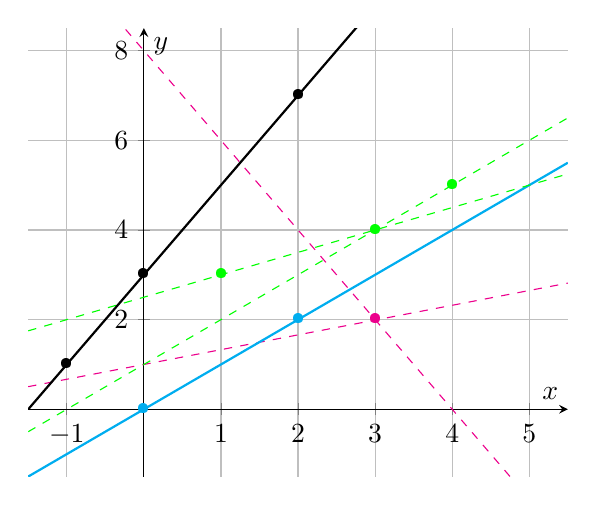
\begin{tikzpicture}
    \begin{axis}[
        axis x line=center,
        xlabel={$x$},
        axis y line=center,
        ylabel={$y$},
        xmin=-1.5,
        xmax=5.5,
        ymin=-1.5,
        ymax=8.5,
        grid,
    ]
        % part a
        \node [magenta] (point-a1) at (axis cs: 3,2) {\textbullet};
        \addplot[domain=-1.5:5.5,samples=50,mark=none,magenta,dashed]{-2*x+8};
        \addplot[domain=-1.5:5.5,samples=50,mark=none,magenta,dashed]{.33*x+1};
        % part b
        \node [cyan] (point-b1) at (axis cs: 0,0) {\textbullet};
        \node [cyan] (point-b2) at (axis cs: 2,2) {\textbullet};
        \addplot[domain=-1.5:5.5,samples=50,mark=none,cyan,thick]{x};
        % part c
        \node [green] (point-c1) at (axis cs: 1,3) {\textbullet};
        \node [green] (point-c2) at (axis cs: 3,4) {\textbullet};
        \node [green] (point-c3) at (axis cs: 4,5) {\textbullet};
        \addplot[domain=-1.5:5.5,samples=50,mark=none,green,dashed]{.5*x+2.5};
        \addplot[domain=-1.5:5.5,samples=50,mark=none,green,dashed]{x+1};
        % part d
        \node (point-d1) at (axis cs: -1,1) {\textbullet};
        \node (point-d2) at (axis cs: 0,3) {\textbullet};
        \node (point-d3) at (axis cs: 2,7) {\textbullet};
        \addplot[domain=-1.5:5.5,samples=50,mark=none,thick]{2*x+3};
    \end{axis}
    \end{tikzpicture}
    \end{center}

    \renewcommand{\labelenumi}{(\alph{enumi})} 
    \begin{enumerate}
        \item No; there are not enough points to define a \emph{unique} degree-1 polynomial, and in fact there are infinitely many degree-1 polynomials passing through this point. (In \textcolor{magenta}{pink} above.)
        \item Yes; these points uniquely define the polynomial $f(x) = x$. (In \textcolor{cyan}{light blue} above.)
        \item No; there is no degree-1 polynomial passing through these points because they are not properly aligned. However, they do define a unique degree-2 polynomial. (In \textcolor{green}{green} above.)
        \item Yes; these points uniquely define the polynomial $f(x) = 2x + 3$. (In black above.)
    \end{enumerate}
\end{answer}

\subsubsection{Lagrange Interpolation*}
\begin{answer}
    \renewcommand{\labelenumi}{(\alph{enumi})}
    \begin{enumerate}
        \item $2(1) + 2(2) + 2(3) + 2(4) + 2(5) = 2(1+2+3+4+5) = 2(15) = 30$
        \item $1+1+1+1+1 = 5(1) = 5$
        \item $1+5+(-3)+0+8 = 11$
        \item $1+5+(-3)=3$
    \end{enumerate}
\end{answer}

\begin{answer}
    \renewcommand{\labelenumi}{(\alph{enumi})}
    \begin{enumerate}
        \item $2(1) \cdot 2(2) \cdot 2(3) \cdot 2(4) \cdot 2(5) = 2^5\cdot1\cdot2\cdot3\cdot4\cdot5 
        = 32\cdot120 = 3840$
        \item $1\cdot1\cdot1\cdot1\cdot1 = 1$
        \item $1\cdot5\cdot(-3)\cdot0\cdot8 = 0$
        \item $1\cdot5\cdot(-3) = -15$
    \end{enumerate}
\end{answer}

\begin{answer}
    \renewcommand{\labelenumi}{(\alph{enumi})}
    \begin{enumerate}
        \item $x_0 = 0$:
        \begin{align*}
            \ell_0(0) &= \frac{(0-1)(0-4)}{4} = \frac{(-1)(-4)}{4} &= 1\\
            \ell_1(0) &= \frac{0(0-4)}{-3} = \frac{0(-4)}{-3} &= 0\\
            \ell_2(0) &= \frac{0(0-1)}{12} = \frac{0(-1)}{12} &= 0
        \end{align*}
        \item $x_1 = 1$:
        \begin{align*}
            \ell_0(1) &= \frac{(1-1)(1-4)}{4} = \frac{(0)(-3)}{4} &= 0\\
            \ell_1(1) &= \frac{1(1-4)}{-3} = \frac{1(-3)}{-3} &= 1\\
            \ell_2(1) &= \frac{1(1-1)}{12} = \frac{1(0)}{12} &= 0
        \end{align*}
        \item $x_2 = 4$:
        \begin{align*}
            \ell_0(4) &= \frac{(4-1)(4-4)}{4} = \frac{(3)(0)}{4} &= 0\\
            \ell_1(4) &= \frac{4(4-4)}{-3} = \frac{4(0)}{-3} &= 0\\
            \ell_2(4) &= \frac{4(4-1)}{12} = \frac{4(3)}{12} &= 1
        \end{align*}
    \end{enumerate}
\end{answer}

\begin{answer}
    $3x^2 + 7x - 12$
\end{answer}

\begin{answer}
    N/A
\end{answer}

\begin{answer}
    N/A
\end{answer}